%%%%%%%%%%%%%%%%%%%%%%%%%%%%%%%%%%%%%%%%%%%%%%%%%%%%%%%%%%%%%%%%%%%%%
% LaTeX Template: Project Titlepage Modified (v 0.1) by rcx
%
% Original Source: http://www.howtotex.com
% Date: February 2014
% 
% This is a title page template which be used for articles & reports.
% 
% This is the modified version of the original Latex template from
% aforementioned website.
% 
%%%%%%%%%%%%%%%%%%%%%%%%%%%%%%%%%%%%%%%%%%%%%%%%%%%%%%%%%%%%%%%%%%%%%%

\documentclass[12pt]{report}
\usepackage[a4paper]{geometry}
\usepackage[myheadings]{fullpage}
\usepackage{fancyhdr}
\usepackage{lastpage}
\usepackage{graphicx, wrapfig, subcaption, setspace, booktabs}
\usepackage[T1]{fontenc}
\usepackage[font=small, labelfont=bf]{caption}
\usepackage{fourier}
\usepackage[protrusion=true, expansion=true]{microtype}
\usepackage[english]{babel}
\usepackage{sectsty}
\usepackage{url, lipsum}
\usepackage{color}
\usepackage{hyperref}
\usepackage{array}
\usepackage{supertabular}
\usepackage{hhline}
\usepackage{enumitem}
\usepackage{graphicx}

\newcommand{\HRule}[1]{\rule{\linewidth}{#1}}
\renewcommand{\theenumii}{\arabic{enumii}.}
\addto\captionsenglish{
  \renewcommand{\contentsname}
    {Innhold}
}
\onehalfspacing
\setcounter{tocdepth}{5}
\setcounter{secnumdepth}{5}

%-------------------------------------------------------------------------------
% HEADER & FOOTER
%-------------------------------------------------------------------------------
\pagestyle{fancy}
\fancyhf{}
\setlength\headheight{15pt}
\fancyhead[L]{Skriv navn her} %TODO
\fancyhead[R]{}
\fancyfoot[R]{Page \thepage\ of \pageref{LastPage}}
%-------------------------------------------------------------------------------
% TITLE PAGE
%-------------------------------------------------------------------------------

\begin{document}

\title{ \normalsize \textsc{}
		\\ [2.0cm]
		\HRule{0.5pt} \\
		\LARGE \textbf{\uppercase{Bruksm{\O}nsterdiagram og bruksm{\O}nstertekst}}
		\HRule{2pt} \\ [0.5cm]
		\normalsize \today \vspace*{5\baselineskip}}

\date{}

\author{
		Skriv navn her  \\  %TODO
		Universitetet i Bergen \\
		Informatikk }

\maketitle
\tableofcontents
\newpage

%-------------------------------------------------------------------------------
% Section title formatting
\sectionfont{\scshape}
%-------------------------------------------------------------------------------

%-------------------------------------------------------------------------------
% BODY
%-------------------------------------------------------------------------------

\section*{Matkrig}
\addcontentsline{toc}{section}{Matkrig}

\subsection*{Bruksm{\o}nstertekst:}
\addcontentsline{toc}{subsection}{Bruks{\o}nstertekst:}

\subsubsection*{Hovedflyt:}
\begin{enumerate}
\item Akt{\o}r n f{\aa}r 30 sekunder p{\aa} {\aa} bevege seg fritt p{\aa} kartet. 
\item Akt{\o}r n velger v{\aa}pen 
\item Akt{\o}r n velger retning 
\item Akt{\o}r n velger kraft for lenge
\item Systemet registrer prosjektilposisjon 
\item Systemet endrer milj{\o}et ut ifra prosjektilkraft og type 
\item Motstander blir truffet av prosjektil 
\item Systemet beregner motstanders helse minus skaden som ble utgjort
\item Motstander mister helsepoeng 
\item Motstander d{\o}r
\item Gjenst{\aa}ende spiller vinner
\end{enumerate}

\subsubsection*{Alternativ handlinger:}

\begin{enumerate}[label=\Alph*]
\item 
\bigskip

\begin{enumerate}
\item @1 Akt{\o}r beveger seg ut av kartet 
\item Gjenoppta @11 
\end{enumerate}
\item 
\bigskip

\begin{enumerate}
\item @2 Akt{\o}r har ikke ammunisjon 
\item Gjenoppta @2 
\end{enumerate}
\item 
\bigskip

\begin{enumerate}
\item @9 Motstander overlever 
\item Gjenoppta @1 
\end{enumerate}
\item 
\bigskip

\begin{enumerate}
\item @Everywhere Rundetiden g{\aa}r ut 
\item Akt{\o}r med mest gjenst{\aa}ende helsepoeng vinner
\end{enumerate}
\item 
\bigskip

\begin{enumerate}
\item @2 Tid for {\aa} velge v{\aa}pen/retning/kraft g{\aa}r ut 
\item Akt{\o}r f{\aa}r ikke angrepet 
\item Gjenoppta @1
\end{enumerate}
\end{enumerate}

\subsection*{Bruksm{\o}nsterdiagram:}
\addcontentsline{toc}{subsection}{Bruksm{\o}nsterdiagram:}

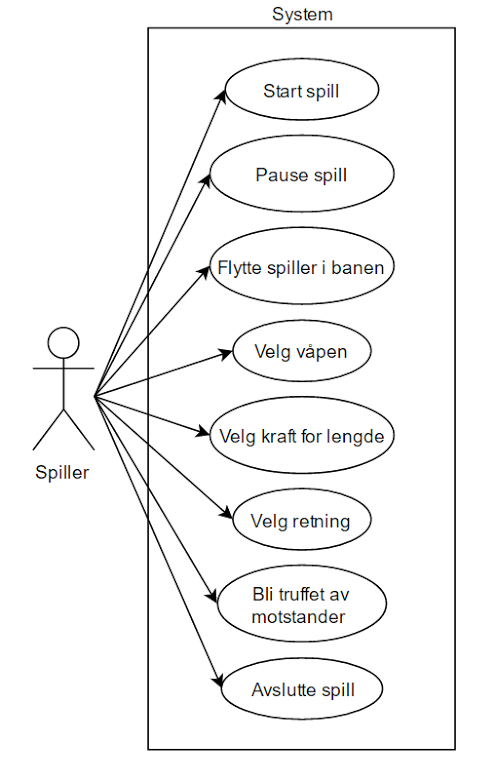
\includegraphics[width=0.8\textwidth,natwidth=610,natheight=642]{use_case_diagram_m.png}



\section*{Spooks}
\addcontentsline{toc}{section}{Spooks}

\subsection*{Bruksm{\o}nstertekst:}
\addcontentsline{toc}{subsection}{Bruks{\o}nstertekst:}

\textbf{Overview}: Spillet starter, du befinner deg i et hus. Du vet ikke hvor du er,
og m{\aa} komme deg ut av huset. 
\bigskip \\
\textbf{Actors}: Spiller, Maskin 
\bigskip \\
\textbf{Pre-conditions:} Spillet er startet p{\aa} en datamaskin

\subsubsection*{Hovedflyt:}

\begin{enumerate}
\item Meny (Start - load game - options - quit)
\item Spiller velger {\aa} starte ett nytt spill
\item Systemet oppretter et nytt spill
\item Systemet starter en klokke som teller ned fra * minutter
\item Spiller trykker p{\aa} et objekt i spillet
\item Spiller f{\aa}r objektet
\item Systemet legger tingen i Spillerens inventory
\end{enumerate}

\textit{Steg 4-7 g{\aa}r i loop til Spiller har riktig objekt (evt. l{\o}st en g{\aa}te) til {\aa} g{\aa} videre neste
rom}

\begin{enumerate}[resume]
\item Spiller velger objekt fra inventory
\item Systemet markerer objekt i inventoryen
\item Spiller bruker objektet p{\aa} d{\o}ren
\item Systemet {\aa}pner d{\o}ren
\item Spiller klikker p{\aa} d{\o}ren
\item Systemet fytter spilleren til neste rom (niv{\aa})
\end{enumerate}

\textit{Steg 4-13 g{\aa}r i loop til Spiller har funnet {\textquotedbl}hovedn{\o}kkel/-objekt`` (til {\aa} komme seg ut
av huset)}

\begin{enumerate}[resume]
\item Spiller plukker opp {\textquotedbl}hovedn{\o}kkel{\textquotedbl}
\item Systemet legger {\textquotedbl}hovedn{\o}kkel{\textquotedbl} i inventory
\item Spiller velger {\textquotedbl}hovedn{\o}kkel{\textquotedbl} fra inventory
\item Systemet markerer {\textquotedbl}hovedn{\o}kkel{\textquotedbl} i inventory
\item Spiller klikker p{\aa} utgangsd{\o}ren
\item Systemet {\aa}pner d{\o}ren
\item Systemet forteller Spilleren at Spiller vant
\item Systemet returnerer til hovedmeny
\end{enumerate}

\subsubsection*{Alternative handlinger:}

\begin{enumerate}[label=\Alph*]
\item 
\bigskip

\begin{enumerate}
\item @2 Spiller velger {\aa} avslutte spillet
\item Systemet avslutter spillet
\end{enumerate}
\item 
\bigskip

\begin{enumerate}
\item @2 Spiller velger {\aa} starte spillet fra et lagret punkt
\item Systemet laster opp et lagret spill
\item Spilleren begynner fra lagret spill
\end{enumerate}
\item 
\bigskip

\begin{enumerate}
\item @5 Spiller pr{\o}ver {\aa} trykke p{\aa} et ugyldig objekt
\item Systemet gir Spiller beskjed om at objektet er ugyldig (vha lyd ect.) Ingenting skjer med objektet
\item Gjennoppta @5
\end{enumerate}
\item 
\bigskip

\begin{enumerate}
\item @4, 6, 8, 10, 12, 14, 16, 18 tiden g{\aa}r ut
\item Systemet fjerner alle objekter fra inventory
\item Systemet plasserer Spiller i utgangspunktrommet
\item Gjennoppta @4
\end{enumerate}
\end{enumerate}

\subsection*{Bruksm{\o}nsterdiagram:}
\addcontentsline{toc}{subsection}{Bruksm{\o}nsterdiagram:}

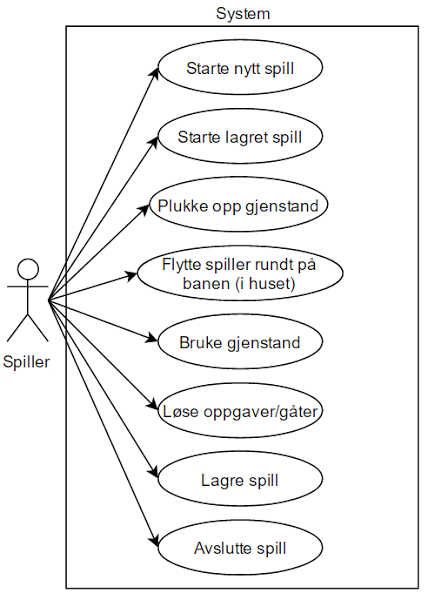
\includegraphics[width=0.8\textwidth,natwidth=610,natheight=642]{use_case_diagram_s.png}



\section*{Tower Defence Uteliv}
\addcontentsline{toc}{section}{Tower Defence Uteliv}

\subsection*{Bruksm{\o}nstertekst:}
\addcontentsline{toc}{subsection}{Bruks{\o}nstertekst:}

\subsection*{Bruksm{\o}nsterdiagram:}
\addcontentsline{toc}{subsection}{Bruksm{\o}nsterdiagram:}




\section*{Bilspill}
\addcontentsline{toc}{section}{Bilspill}

\subsection*{Bruksm{\o}nstertekst:}
\addcontentsline{toc}{subsection}{Bruks{\o}nstertekst:}

\subsection*{Bruksm{\o}nsterdiagram:}
\addcontentsline{toc}{subsection}{Bruksm{\o}nsterdiagram:}




\end{document}

%-------------------------------------------------------------------------------
% SNIPPETS
%-------------------------------------------------------------------------------

%\begin{figure}[!ht]
%	\centering
%	\includegraphics[width=0.8\textwidth]{file_name}
%	\caption{}
%	\centering
%	\label{label:file_name}
%\end{figure}

%\begin{figure}[!ht]
%	\centering
%	\includegraphics[width=0.8\textwidth]{graph}
%	\caption{Blood pressure ranges and associated level of hypertension (American Heart Association, 2013).}
%	\centering
%	\label{label:graph}
%\end{figure}

%\begin{wrapfigure}{r}{0.30\textwidth}
%	\vspace{-40pt}
%	\begin{center}
%		\includegraphics[width=0.29\textwidth]{file_name}
%	\end{center}
%	\vspace{-20pt}
%	\caption{}
%	\label{label:file_name}
%\end{wrapfigure}

%\begin{wrapfigure}{r}{0.45\textwidth}
%	\begin{center}
%		\includegraphics[width=0.29\textwidth]{manometer}
%	\end{center}
%	\caption{Aneroid sphygmomanometer with stethoscope (Medicalexpo, 2012).}
%	\label{label:manometer}
%\end{wrapfigure}

%\begin{table}[!ht]\footnotesize
%	\centering
%	\begin{tabular}{cccccc}
%	\toprule
%	\multicolumn{2}{c} {Pearson's correlation test} & \multicolumn{4}{c} {Independent t-test} \\
%	\midrule	
%	\multicolumn{2}{c} {Gender} & \multicolumn{2}{c} {Activity level} & \multicolumn{2}{c} {Gender} \\
%	\midrule
%	Males & Females & 1st level & 6th level & Males & Females \\
%	\midrule
%	\multicolumn{2}{c} {BMI vs. SP} & \multicolumn{2}{c} {Systolic pressure} & \multicolumn{2}{c} {Systolic Pressure} \\
%	\multicolumn{2}{c} {BMI vs. DP} & \multicolumn{2}{c} {Diastolic pressure} & \multicolumn{2}{c} {Diastolic pressure} \\
%	\multicolumn{2}{c} {BMI vs. MAP} & \multicolumn{2}{c} {MAP} & \multicolumn{2}{c} {MAP} \\
%	\multicolumn{2}{c} {W:H ratio vs. SP} & \multicolumn{2}{c} {BMI} & \multicolumn{2}{c} {BMI} \\
%	\multicolumn{2}{c} {W:H ratio vs. DP} & \multicolumn{2}{c} {W:H ratio} & \multicolumn{2}{c} {W:H ratio} \\
%	\multicolumn{2}{c} {W:H ratio vs. MAP} & \multicolumn{2}{c} {\% Body fat} & \multicolumn{2}{c} {\% Body fat} \\
%	\multicolumn{2}{c} {} & \multicolumn{2}{c} {Height} & \multicolumn{2}{c} {Height} \\
%	\multicolumn{2}{c} {} & \multicolumn{2}{c} {Weight} & \multicolumn{2}{c} {Weight} \\
%	\multicolumn{2}{c} {} & \multicolumn{2}{c} {Heart rate} & \multicolumn{2}{c} {Heart rate} \\
%	\bottomrule
%	\end{tabular}
%	\caption{Parameters that were analysed and related statistical test performed for current study. BMI - body mass index; SP - systolic pressure; DP - diastolic pressure; MAP - mean arterial pressure; W:H ratio - waist to hip ratio.}
%	\label{label:tests}
%\end{table}